\documentclass{beamer}
\usepackage[T1]{fontenc}
\usepackage{bookmark}
\usepackage{amsmath}
\usetheme{Berkeley}


\usepackage{amsmath, amssymb,amsthm,mathtools}
\usepackage[shortlabels]{enumitem}
\usepackage{tikz-cd} 
% \usepackage{euler}
\usepackage{tikz}
\usetikzlibrary{positioning}

\newtheorem{prob}{Problem}
\newtheorem{prop}{Proposition}
\newtheorem{cor}{Corollary}
\newtheorem{lem}{Lemma}
\newtheorem{topic}{Topic}
\newtheorem*{opq*}{Open Question}
\newtheorem{thm}{Theorem}
\newtheorem*{thm*}{Theorem}

\theoremstyle{definition}
\newtheorem{exmp}{Example}
\newtheorem*{exmp*}{Example}
\newtheorem*{defn*}{Definition}
\newtheorem{defn}{Definition}
\newtheorem*{rem*}{Remark}
\newtheorem*{ans*}{Answer}
\newtheorem{exc}{Exercise}
\newtheorem*{quest*}{Question}
\newtheorem{quest}{Question}
\newtheorem{obs}{Observation}
\newtheorem{rem}{Remark}
\newtheorem{notn}{Notation}

\newcommand{\inv}{^{-1}}
\newcommand{\norm}[1]{\left\lVert#1\right\rVert}
\newcommand{\Q}{\mathbb{Q}}
\newcommand{\R}{\mathbb{R}}
\newcommand{\Z}{\mathbb{Z}}
\newcommand{\C}{\mathbb{C}}
\newcommand{\N}{\mathbb{N}}
\newcommand{\F}{\mathbb{F}}
\newcommand{\p}{\mathbb{P}}
\newcommand{\fp}{\mathbb{F}_p}
\newcommand{\zp}{\mathbb{Z}_p}
\newcommand{\calm}{\mathcal{M}}
\newcommand{\calu}{\mathcal{U}}
\newcommand{\caln}{\mathcal{N}}
\newcommand{\h}{\mathcal{H}}
\newcommand{\K}{\mathcal{K}}
\newcommand{\I}{\mathcal{I}}
\newcommand{\T}{\mathbb{T}}
\newcommand{\ran}{\textup{ran }}
\newcommand{\vol}{\textup{Vol}}
\newcommand{\diff}{\textup{d}}
\newcommand{\calr}{\mathcal{R}}
\newcommand{\calp}{\mathcal{P}}
\newcommand{\cala}{\mathcal{A}}
\newcommand{\calx}{\mathcal{X}}
\newcommand{\caly}{\mathcal{Y}}
\newcommand{\calz}{\mathcal{Z}}
\newcommand{\call}{\mathcal{L}}
\newcommand{\calb}{\mathcal{B}}
\newcommand{\calf}{\mathcal{F}}
\newcommand{\calg}{\mathcal{G}}
\newcommand{\cale}{\mathcal{E}}
\newcommand{\calc}{\mathcal{C}}
\newcommand{\calk}{\mathcal{K}}
\newcommand{\calh}{\mathcal{H}}
\newcommand{\calt}{\mathcal{T}}
\newcommand{\plv}{\mathcal{v}}
\newcommand{\A}{\mathbb{A}}
\newcommand{\oo}{\mathcal{O}}
\newcommand{\ov}{\mathcal{O}_v}
\newcommand{\ox}{\mathcal{O}_X}
\newcommand{\oy}{\mathcal{O}_Y}
\newcommand{\fv}{\mathbb{F}_v}
\newcommand{\ok}{\mathcal{O}_k}
\newcommand{\oks}{\mathcal{O}_{k,S}}
\newcommand{\mf}{\mathfrak}
\newcommand{\ovg}{\overline{\gamma}}
\newcommand{\zplane}{\A^2_\Z}
\newcommand{\zline}{\A^1_\Z}
\newcommand{\spec}{\textup{Spec}}
\newcommand{\proj}[1]{\textup{Proj}(#1)}
\newcommand{\Max}{\textup{Max}}
\newcommand{\inj}{\xhookrightarrow{}}
\newcommand{\surj}{\twoheadrightarrow}
\newcommand{\finpl}{\Omega_{k,f}}
\newcommand{\Kbar}{\overline{K}}
\newcommand{\kbar}{\overline{k}}
\newcommand{\gal}{\textup{Gal}}
\newcommand{\oxx}{\mathcal{O}_{X,x}}
\newcommand{\oxi}{\mathcal{O}_{X,{\xi}}}
\newcommand{\oxy}{\mathcal{O}_{X,y}}
\newcommand{\oyy}{\mathcal{O}_{Y,y}}
\newcommand{\oxp}{\mathcal{O}_{X,{\mf{p}}}}
\newcommand{\Hom}{\textup{Hom}}
\newcommand{\Frac}{\textup{Frac}}
\newcommand{\im}{\textup{Im }}
\newcommand{\id}{\textup{Id}}
\newcommand{\rad}{\textup{Rad}}
\newcommand{\Ker}[1]{\textup{Ker}(#1)}
\newcommand{\mor}[2]{\textup{Mor}(#1,#2)}
\newcommand{\Mor}[3]{\textup{Mor}_{#1}(#2,#3)}
\newcommand{\tens}[3]{#2 \otimes_{#1} #3}
\newcommand{\fib}[3]{#2 \times_{#1} #3}
\newcommand{\iso}{\tilde{\longrightarrow}}
\newcommand{\irr}[2]{\textup{Irr}^1_{#1/#2}}
\newcommand{\qncyc}{\Q_n}
\newcommand{\qnncyc}{\Q_{n-1}}
\newcommand{\qnnncyc}{\Q_{n-2}}
\newcommand{\resga}{\mathbf{R}_{A/K}\ga{A}}
\newcommand{\resgal}{\mathbf{R}_{L/K}\ga{L}}
\newcommand{\resgm}{\mathbf{R}_{A/K}\gm{A}}
\newcommand{\md}{\mathbf{m}_d}
\newcommand{\disc}{\textup{disc}}
\newcommand{\qbar}{\overline{\Q}}
\newcommand{\gm}[1]{\mathbb{G}_{m,#1}}
\newcommand{\ga}[1]{\mathbb{G}_{a,#1}}
\newcommand{\mm}[1]{\mathbf{#1}}
\newcommand{\rk}{\textup{rk}_\Z\,}
\newcommand{\jac}{\textup{Jac}}
\newcommand{\trlk}{\textup{Tr}_{L/K}}
\newcommand{\bij}{\xleftrightarrow{1:1}}

\definecolor{darkgreen}{rgb}{0.0, 0.5, 0.0}
 
\title{MATH 392: Intro to Neural Networks}

 
\author{Arvind Suresh}

\date[Dec 11, 2024]
 {Dec 11, 2024}

\begin{document}

\frame{\titlepage} % # 1
\section[Outline]{}
\frame{\tableofcontents}

% Sections:

%Section 1. What is AI, anyway?

% Section 2. What is (supervised) machine learning?

% Second slide will proceed as follows.
% We will explain that in practice, we first analyze the data to hypothesize a model (i.e. a parametric class of functions) for the true function.
%We provide a simple example of a linear regression model to predict house prices from square footage.
%We provide a simple example of a logistic regression model to predict whether a student will pass or fail a test based on the number of hours they studied.

% 3. What is a neural network?
% 4. MATH 392: Learning objectives
% 5. MATH 392: Course structure
% 6. MATH 392: Reasons why you might like to enroll

\section{What is AI, anyway?}
 
\frame
{\frametitle{What is AI, anyway?}

\vspace{0.1in}
% This section will take up exactly one slide. 
% We will first explain that modern AI's like ChatGPT are based on so called Large Language Models (LLMs). 
% We will summarize how LLM's work, namely-- they input a sequence of words, and output a sequence of words.
% Finally, we will mention that the output is generated word-by-word, and that the model is trained to generate the most likely word next.

\begin{enumerate}[$\bullet$]
    \item Modern AI's like ChatGPT are based on so called \textbf{Large Language Models} (LLMs). \vspace{0.1in} 
    \pause
    \item These are very sophisticated programs-- given an input (``prompt''), they generate an output (a textual response, image, and so on). \vspace{0.1in} 
    \pause
    \item For text, output is generated word-by-word:
    
    The model is trained to generate the \emph{most likely} word next, given the words that have come before.\vspace{0.1in}
    \pause
    \item Thus,  LLM's are in the business of making \emph{predictions}. \vspace{0.1in} 
    \pause
    \item So, at its core, modern AI falls within the framework of \textbf{machine learning} (ML).
\end{enumerate}

\vspace{0.15in}
}

\section{What is ML?}
% This section will take up two slides.

\frame{\frametitle{Framework of ML}

% On the first slide, we will explain the over-arching framework of (supervised) machine learning as follows-- we will explain that we have a certain target variable that we want to predict, and that we have a set of input variables that we can use to predict the target variable.
% We will explain that the goal of machine learning is to find "the one true function" that maps the input variables to the target variable.

\begin{enumerate}[$\bullet$]
    \item \textbf{Given}: a \emph{dataset} (matrix): \pause
        \begin{enumerate}[$\circ$]
            \item Some columns $X_1, \dotsc, X_m$ are \emph{features/predictors}. \pause
            \item One column $Y$ is the \emph{target variable}. \pause
            \item Each row is a \emph{data point} (features and target). \vspace{0.1in} \pause
        \end{enumerate}         
    \item \textbf{Believe}: the target can be predicted from the features, i.e. there is a ``one true function'' $F$ such that
    \begin{equation*}
        Y = F(X_1, \dotsc, X_m) + \textup{(noise)}. 
    \end{equation*} \pause %delete vspace
    \vspace{-0.2in}
    \item \textbf{Goal}: \emph{Learn $F$\dots} \pause i.e. find a \emph{good approximation} to $F$. \vspace{0.1in} \pause
    \item \textbf{Model}: A class of functions that we belive might approximate $F$ (e.g. linear, polynomial, logistic). \vspace{0.1in}\pause
    \item \textbf{Training}: \emph{Fit the model} to the given data to get the best approximation to $F$ within our class.
\end{enumerate}
}
 
 \frame% # 2
{\frametitle{The simplest example of a ML model}

Choosing a model amounts to choosing a type of ``formula'' for our approximation of $F$.

\begin{example}[Linear models]
\begin{enumerate}[$\bullet$]
    \item \textbf{Goal}: Predict house prices ($Y$) from square footage ($X$). \pause
    \item \textbf{Belief}: $Y = m X + b + \textup{(noise)}$. \pause
    \item \textbf{Model parameters}: $m$ and $b$. \pause
    \item \textbf{Training}: Find the values of $m$ and $b$ that best fit the data. \pause 
    
    Get the best approximation to $F$ among all linear functions: 
    \begin{equation*}
        f(X) = \hat{m} X + \hat{b}.
    \end{equation*} \pause
    \vspace{-0.25in}
    \item \textbf{Prediction}: Given a house with a certain square footage $x$, predict the house price to be $y = f(x) = \hat{m} x + \hat{b}$.
\end{enumerate}
\end{example}
}

\section{What is a NN?}

\frame% # 2
{\frametitle{What are neural networks?}
% Create a simple diagram of a neural network with 1 input layer, 1 hidden layer, and 1 output layer.
\begin{equation*}
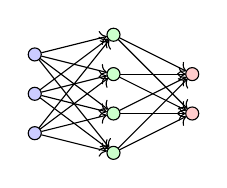
\begin{tikzpicture}[scale=0.5, transform shape]
    % Input layer
    \foreach \i in {1,...,3}
        \node[circle, draw, fill=blue!20] (I\i) at (0,-\i) {};

    % Hidden layer
    \foreach \i in {1,...,4}
        \node[circle, draw, fill=green!20] (H\i) at (2,-\i+0.5) {};

    % Output layer
    \foreach \i in {1,...,2}
        \node[circle, draw, fill=red!20] (O\i) at (4,-\i-0.5) {};

    % Connect input layer to hidden layer
    \foreach \i in {1,...,3}
        \foreach \j in {1,...,4}
            \draw[->] (I\i) -- (H\j);

    % Connect hidden layer to output layer
    \foreach \i in {1,...,4}
        \foreach \j in {1,...,2}
            \draw[->] (H\i) -- (O\j);
\end{tikzpicture}
\end{equation*}
\begin{enumerate}[$\bullet$]
    \item A flexible class of ML models that combine linear and non-linear functions in \emph{layers}:
    \begin{center}
    {\color{blue} \emph{Input layer}} $\longrightarrow$ {\color{darkgreen} \emph{Hidden layers}} $\longrightarrow$ {\color{red} \emph{Output layer}}
    \end{center} \vspace{0.05in}\pause
    \item Inspired by biology-- the data flow in a NN is similar to how neurons transmit info by electric impulses. \vspace{0.05in}\pause
    \item The model parameters are called \emph{weights}; they are trained using a process called \emph{backpropagation}. \vspace{0.05in} \pause
    \item LLMs like ChatGPT are based on neural networks with billions of weights! \vspace{0.05in} 
\end{enumerate}
}

\frame
{\frametitle{Why are neural networks so useful?}
There are two reasons, one theoretical, one computational. \vspace{0.1in} \pause
\begin{enumerate}[$\bullet$]
    \item (Theoretical): They are \emph{universal approximators}, which means that  \emph{any} real-world function $F$ can (in principle) be closely approximated by a NN. \vspace{0.2in} \pause
    \item (Computational): They are \emph{scalable}, which means that they can be trained on large datasets with many features. \vspace{0.1in} \pause
    
    Highly optimized hardware (GPUs) and software (e.g. PyTorch) allow for large-scale parallel computations.
\end{enumerate}
}
\section{Learning objectives}

\frame
{\frametitle{MATH 392: Learning objectives}

% Understand the key mathematical concepts used in neural networks, including linear
% algebra, gradient descent, and backpropagation.
% • Learn to build and implement simple neural networks using libraries like PyTorch.
% • Analyze and evaluate neural network models, with an emphasis on model optimization,
% regularization, and hyperparameter tuning.
% • Gain experience in the research method (namely, asking questions and being able to
% hunt down answers or resources).
% • Prepare for independent research by developing the ability to approach problems related
% to neural networks and machine learning with a solid mathematical framework.
\begin{enumerate}[$\bullet$]
    \item Gain experience in the research method (asking questions and hunting for answers). \vspace{0.1in} \pause
    \item Develop a solid mathematical foundation to approach problems related to NNs: linear algebra, probability and statistics, gradient descent (vector calculus). \vspace{0.1in} \pause
    \item Learn to build and implement simple NNs using libraries like PyTorch. \vspace{0.1in} \pause
    \item Learn how to evaluate NN's (model optimization, regularization, and hyperparameter tuning). \vspace{0.1in} \pause
    \item Demonstrate your learning by completing a final project.
\end{enumerate}
}

\section{Course structure}

\frame
{\frametitle{MATH 392: Course structure}
% Math concepts will be motivated by asking natural questions about datasets provided by
% the instructor.
% • Every week, students will learn key topics and immediately engage with the material
% through hands-on coding exercises (Jupyter notebooks prepared before-hand by the
% instructor).
% • Assignments will primarily consist of mini-projects, implemented in Python using
% industry-standard packages (sklearn and PyTorch).
% • Students will maintain a GitHub repository containing their mini-projects and final project.
% • Students will learn to use GitHub Copilot for Education (free and powerful AI code
% assistant) to write code with minimal effort.
% • Heavy emphasis will be placed on the process of doing research, namely, asking lots of
% interesting questions and collaborating with peers on projects.
\begin{enumerate}[$\bullet$]
    \item \textbf{Motivation}: Develop math concepts by asking natural questions about datasets. \vspace{0.03in} \pause
    \item \textbf{In-class}: Learn key concepts $\longrightarrow$ engage with the material via hands-on coding exercises (Jupyter notebooks). \vspace{0.03in} \pause
    \item \textbf{Coding}: Will make systematic use of GitHub Copilot for Education to write code with minimal effort. \vspace{0.03in} \pause
    \item \textbf{Assignments}: 4-5 Mini-projects implemented in Python using industry-standard packages, and one final project. \vspace{0.03in} \pause
    \item \textbf{GitHub}: Maintain a repository containing mini-projects and final project. \vspace{0.03in} \pause
    \item \textbf{Research-spirit}: Heavy emphasis on asking interesting questions and collaborating with peers on projects.
\end{enumerate}
}

\section{Why enroll?}

\frame
{\frametitle{MATH 392: Reasons why you might like to enroll}

% You are interested in AI and would like a self-contained introduction covering the basics.
% • You are considering internships/jobs in the field of machine learning/AI and would like to
% get started building a portfolio with projects to showcase to potential employers.
% • You enjoy courses that blend theory (from math) with practice (coding).
% • You are a math major looking to fill the “Application Course” credit.

\begin{enumerate}[$\bullet$]
    \item You are interested in AI and would like a self-contained introduction covering the basics. \vspace{0.1in} \pause
    \item You enjoy seeing math concepts from different courses come together in a single course. \vspace{0.1in} \pause
    \item You are considering internships/jobs in the field of ML/AI and would like to get started building a portfolio with projects to showcase to potential employers. \vspace{0.1in} \pause
    \item You enjoy courses that blend theory (from math) with practice (coding). \vspace{0.1in} \pause
    \item You are a math major looking to fill the ``Application Course'' credit.
\end{enumerate}
}

\section{Conclusion}


\frame{
\frametitle{Closing remarks}

I hope you will consider enrolling in MATH 392! \vspace{0.3in}

Please feel free to reach out to me at {\color{blue} \emph{arvindsuresh@arizona.edu}} if you have any questions about the course, or simply want to chat about neural networks (or anything else mathematical, for that matter). \vspace{0.3in}

Thank you for your time!! \vspace{0.3in}

}

\end{document}

   